\chapter{Design}
\epigraph{``Another quote.''}{\vspace{10pt}Another Author}
\label{chapter:design}
\newpage

This chapter presents the developed algorithm/mechanism used to test the hypothesis. The contents of this section vary depending on the research effort
\section{Design criteria used (if needed)}

\subsection{Detailed specific criteria/tool}

\section{Description of the implementation of other algorithms (by other authors) used to test the hypothesis}

\section{Proposed algorithm}

\subsection{Design of the proposed algorithm}
The  specific description of the design algorithm goes in this place, as well as a flow diagram with the description of how it works as seen on \textbf{Figure \ref{fig:proposedalgorithm} }

\begin{figure}
	\begin{center}
		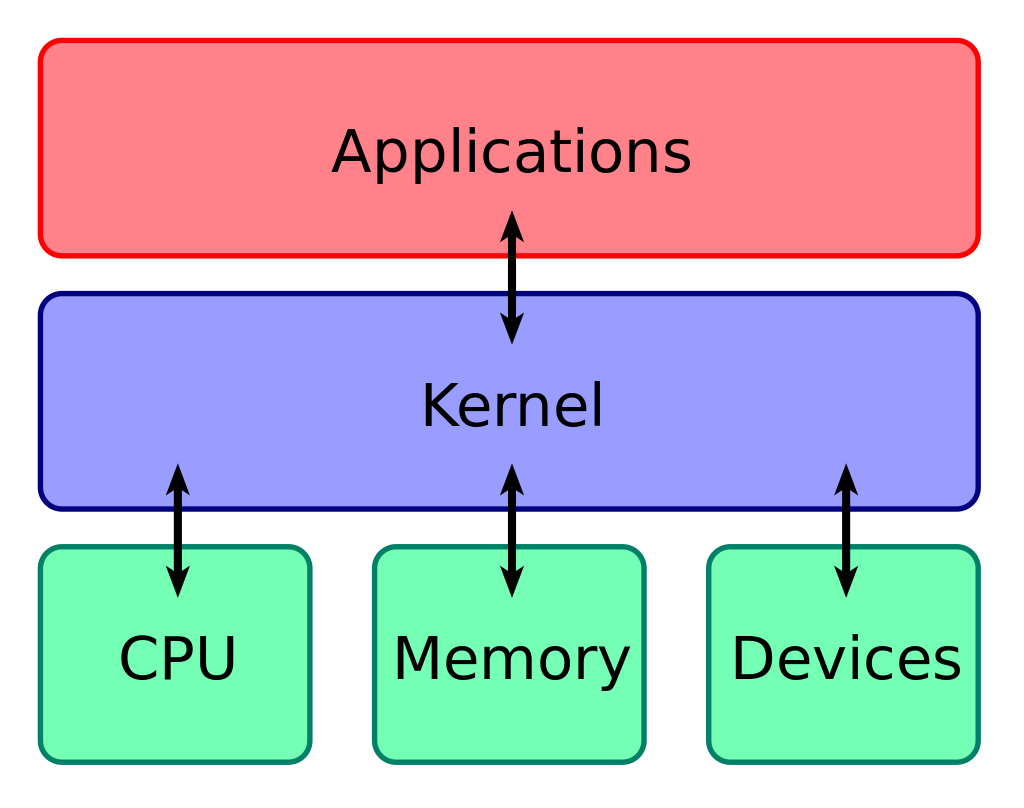
\includegraphics[width=1\columnwidth]{../img/image.png}
		\caption{Example diagram.}
		\label{fig:proposedalgorithm}
	\end{center}
\end{figure} 


\subsection{Limitations and Requirements}
A brief description of the design mechanism's limitations and requirements in accordance with the definitions in Scope and Limitations.


\subsection{Implementation}

A brief description of the implementation and pointer to git where it can be downloaded and tested. \url{https://myalgorithm.com}.
